\section{Diagrammes UML de Connect Four}


\begin{figure}[H]
    \centering
    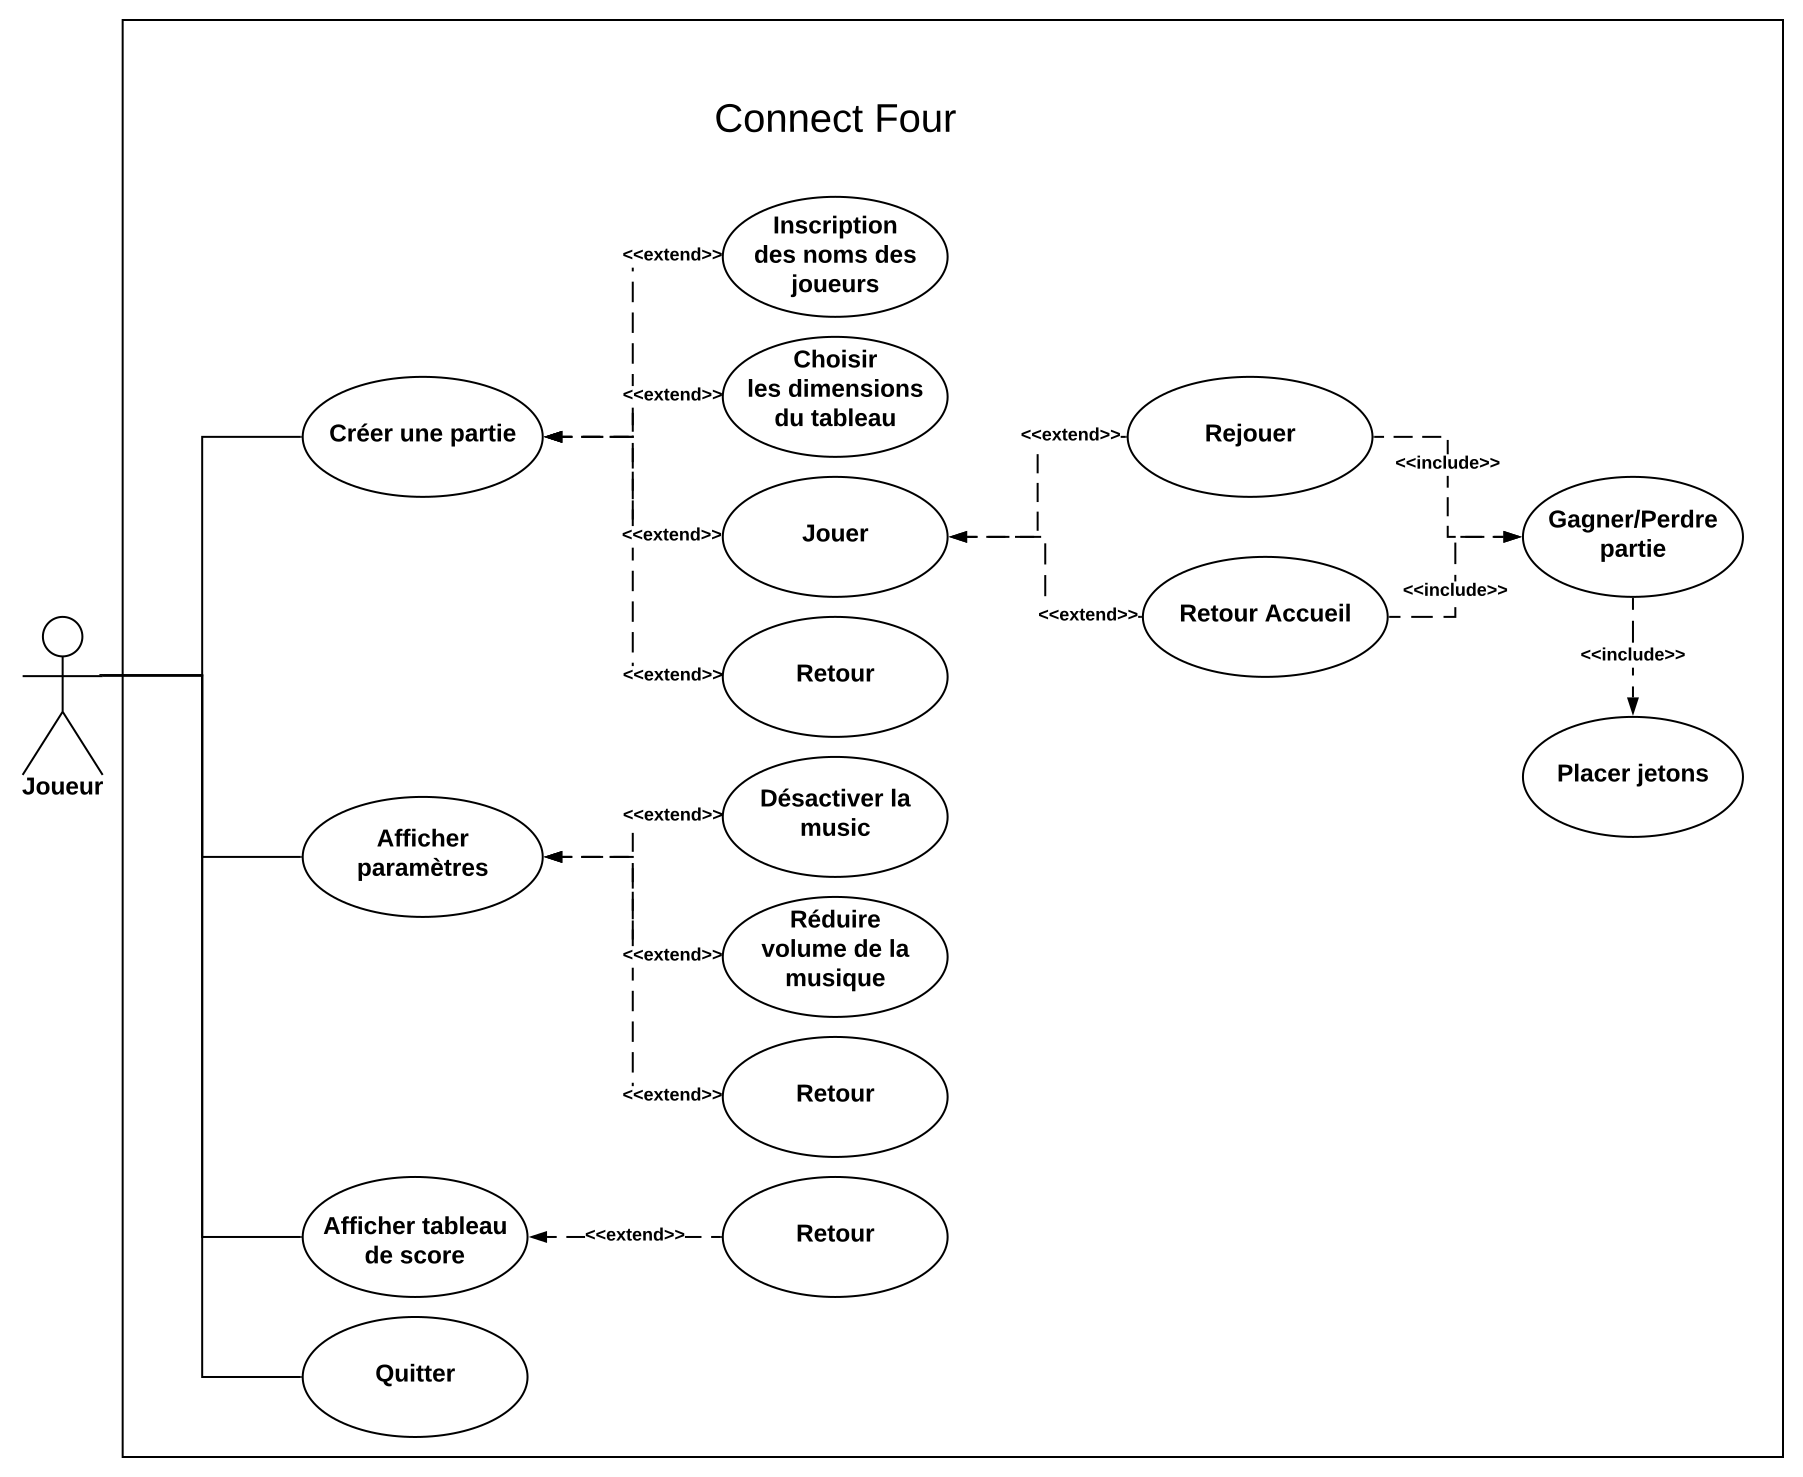
\includegraphics[width=6in]{img/cas}
    \caption{Diagramme de cas d’utilisation UML de haut niveau de Connect Four}
\end{figure}

\begin{figure}[H]
    \centering
    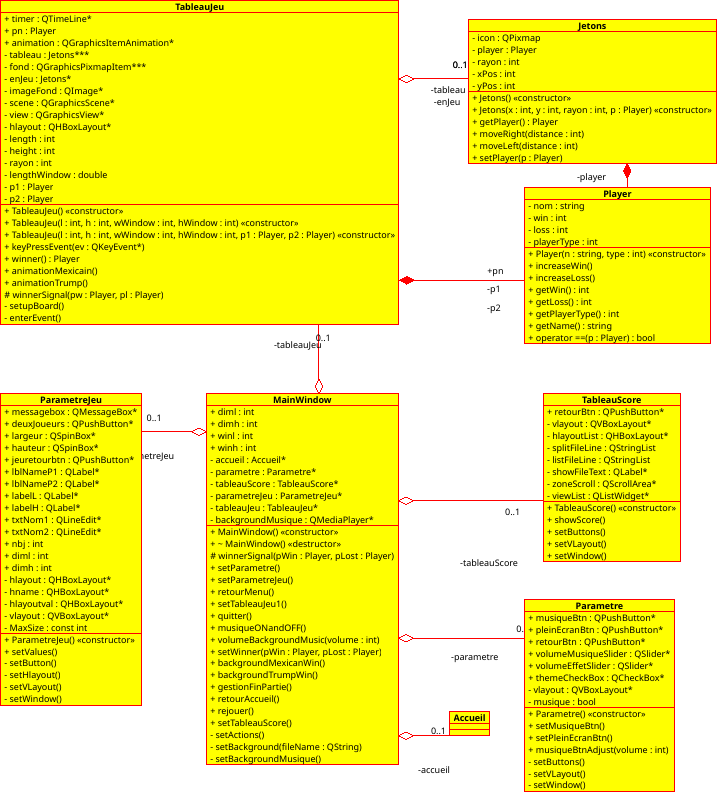
\includegraphics[width=6in]{img/classes}
    \caption{Diagramme de classe de Connect Four}
\end{figure}

\section{Captures d’écrans}

\begin{figure}[H]
    \centering
    
\includegraphics[width=6in]{img/1}
    \caption{Écran 1}
\end{figure}

\begin{figure}[H]
    \centering
    
\includegraphics[width=6in]{img/2}
    \caption{Écran 2}
\end{figure}

\begin{figure}[H]
    \centering
    
\includegraphics[width=6in]{img/3}
    \caption{Écran 3}
\end{figure}

\begin{figure}[H]
    \centering
    
\includegraphics[width=6in]{img/4}
    \caption{Écran 4}
\end{figure}

\section{But, fonctionnement et guide d'usager de Conect Four}

\section{Ergonomie et amélioration}

\section{Plan de tests de Connect Four}

\begin{table}[H]
    \centering
    \caption{Plan de tests de l'interface graphique}
    \begin{tabular}{p{0.25in}p{2.5in}p{0.5in}p{2.5in}}
        \hline
        \bfseries Test & \bfseries Description et résultats & \bfseries Passé & \bfseries Justification \\
        \hline\hline
        1 & Nombre d'élément dans le menu inférieur à 7 & Oui & Tous les menus ont moins de 7 éléments \\
        \hline
    \end{tabular}
\end{table}

\begin{table}[H]
    \centering
    \caption{Plan de tests de l'application}
    \begin{tabular}{p{0.25in}p{2.5in}p{0.5in}p{2.5in}}
        \hline
        \bfseries Test & \bfseries Description et résultats & \bfseries Passé & \bfseries Justification \\
        \hline\hline
        1 & On peux déplacer le pion de gauche à droite & Oui & Le pion se déplace de gauche à droite \\
        2 & Le pion ne peux pas aller à l'extérieur du plateu & Oui & Le déplacement du pion est limité à la largeur du plateau de jeu \\
        3 & Le jeton tombe à l'endroit attendu lorsque qu'on appuie sur la bare d'espacement & Oui & Le pion tombe au bon endroit \\
        \hline
    \end{tabular}
\end{table}
